\problemname{Estimating the Area of a Circle}

One way to estimate the area of a circle is to draw a square that just
encompasses the circle and mark points randomly (with uniform
probability) with a marker. Then, when you get tired of marking points,
count up the number of points that you marked that landed in the circle
and divide it by the total number of points that you marked. That gives
you an idea of how large the circle is relative to the square. Your job
is to judge how accurate this is for given circles and experiment
outcomes.

\begin{figure}
\centering
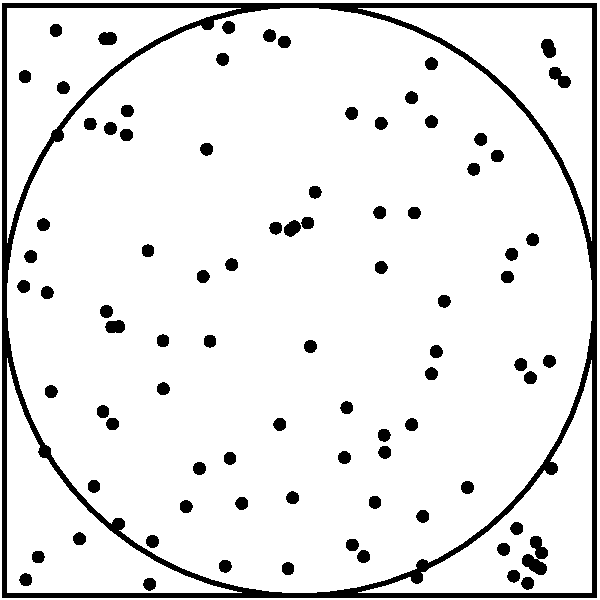
\includegraphics[width=0.3\textwidth,height=0.1\textheight]{circle.pdf}
\caption{An illustration of the random marking process.}
\end{figure}

\newcommand{\tightlist}{}

\begin{itemize}
\item
  this
\item
  is
\item
  a

  \begin{itemize}
  \tightlist
  \item
    superlonglistsuperlonglistsuperlonglistsuperlonglistsuperlonglistsuperlonglistsu
    {[}space{]}perlonglistsuperlonglistsuperlonglistsuperlonglistsuperlonglistsuperlonglistsuperlonglistsuperlonglistsuperlonglistsuperlongl
    {[}new
    line{]}istsuperlonglistsuperlonglistsuperlonglistsuperlonglistsuperlonglistsuperlonglistsuperlonglistsuperlonglistsuperlonglist
  \end{itemize}
\end{itemize}

\hypertarget{input}{%
\subsection{Input}\label{input}}

Input contains up to \(1\,000\) test cases, one test case per line. Each
line has three space-separated numbers: \(r\ m\ c\), where
\(0 < r \le 1\,000\) is a real number with at most \(5\) digits past the
decimal indicating the true radius of the circle,
\(1 \le m \le 100\,000\) is an integer indicating the total number of
marked points, and \(0 \le c \le m\) is an integer indicating the number
of marked points that fall in the circle. Input ends with a line
containing three zeros, which should not be processed.

\hypertarget{output}{%
\subsection{Output}\label{output}}

For each test case, print a line containing two numbers: the true area
of the circle and the estimate according to the experiment. Both numbers
may have a relative error of at most \(10^{-5}\).
